
%--------------------------------------------------------------------------------------%
\frame{
	\frametitle{ Binomial Example 1 }
	(Revision from Last Class)\\
	Suppose a die is tossed 5 times. What is the probability of getting exactly 2 fours?
	
	\textbf{Solution:} This is a binomial experiment in which the number of trials is equal to 5, the number of successes is equal to 2, and the probability of success on a single trial is 1/6 or about 0.167. 
	\\
	\bigskip
	Therefore, the binomial probability is:
	
	\[P(X=2) = ^5C_2 \times (1/6)^2 \times (5/6)^3 = 0.161\]
}

%--------------------------------------------------------------------------------------%
\frame{
	\frametitle{ Binomial Example 2 }
	Suppose there is a container that contains 6 items.  The probability that any one of these items is defective is 0.3. Suppose all six items are inspected. 
	\begin{itemize}
		\item What is the probability of 3 defective components?
		\item What is the probability of 4 defective components?
	\end{itemize}
	
	\[ P(3\text{ defects}) = f(3) = P(X = 3) = {6\choose 3}0.3^3 (1-0.3)^{6-3} = 0.1852 \]
	\[ P(4\text{ defects}) = f(4) = P(X = 4) = {6\choose 4}0.3^4 (1-0.3)^{6-4} = 0.0595 \]
}

%------------------------------------------------------------------%
\frame{
	\frametitle{Binomial Expected Value and Variance}
	
	
	If the random variable X has a binomial distribution with parameters n
	and p, we write
	\[ X \sim B(n,p) \]
	
	Expectation and Variance
	If $X \sim B(n,p)$, then:
	
	\begin{itemize}
		\item Expected Value of X : E(X) = np
		\item Variance of X : Var(X) = np(1-p)
	\end{itemize}
}
%---------------------------------------------------------------------%
\begin{frame}
	\frametitle{Binomial Distribution: Example 1}
	\begin{itemize} \item Diagrams of the probability mass functions of the two binomial
		distributions $B(10, 0.5)$ and $B(10, 0.25)$ are shown in the bar-plots (next slide). \item Which
		is which? Give a reason for your answer.
	\end{itemize}
\end{frame}
%---------------------------------------------------------------------%
\begin{frame}
	\frametitle{Binomial Distribution}
	\begin{figure}
		% Requires \usepackage{graphicx}
		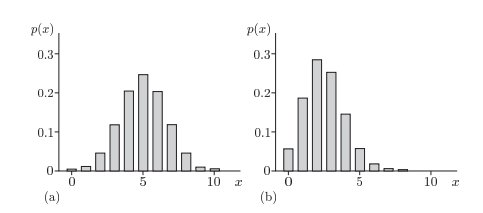
\includegraphics[scale=0.60]{4ABarCharts.jpg}\\
		\caption{Bar Charts}
	\end{figure}
\end{frame}
%---------------------------------------------------------------------%
\begin{frame}
	\frametitle{Binomial Distribution: Example 1}
	\begin{itemize}
		\item Clearly. Figure A is $B(10, 0.5)$ and Figure B is $B(10, 0.25)$.
		\item The mean of B(10, 0.5) is 5, and the mean of B(10, 0.25) is 2.5. These values correspond to the apex of both distributions on the previous slide.
		\item Also the variance of a binomial distribution corresponding to $B(10, 0.25)$ is $1.875$, while for $B(10, 0.25)$ it is $2.500$.
		\item A visual inspection of the two bar-charts would indicate that Figure A has the higher variance.
	\end{itemize}
\end{frame}
%---------------------------------------------------------------------%
\begin{frame}
	\frametitle{Binomial Distribution: Example 2}
	\textbf{Example}
	\begin{itemize}
		\item Components are placed into containers containing 100 items.
		\item After an inspection of a large number of containers the average number of defective items was found to be 10 with a standard deviation of three.
		\item Is the binomial distribution a good useful distribution, given the observed data?
	\end{itemize}
\end{frame}
%---------------------------------------------------------------------%
\begin{frame}
	\frametitle{Binomial Distribution: Example 2}
	
	\begin{itemize}
		\item Let the number of containers be the number of independent trials is $n=100$.
		\item A success may be defined as a defective component.
		\item The probability of a success is approximate $p=0.10$. (The probability of ``failure" is $1-p=0.9$).
		\item The expected number of defective components is $np=10$, which concurs with our observed data.
		\item The variance is computed as \[np(1-p) = 100 \times 0.1 \times 0.9 = 9\]
		\item The observed standard deviation is 3 units, i.e. a variance of 9 square units.
		\item Yes the binomial distribution is useful in this case.
	\end{itemize}
\end{frame}
%============================================================ %
\begin{frame}
	The Binomial distribution is a discrete distribution used.


The outcome of interest is known as a `success'. If we are
interested in how many times we get a six when a dice is rolled.

The probability of success is denoted $p$.

binomial coefficients
\[
\left( {\begin{array}{*{20}c} n \\ k \\ \end{array}} \right) =
\frac{{n!}}{{k!\left( {n - k} \right)!}} \]
\end{frame}
%============================================================ %
\begin{frame}
binomial probability
\[y = \frac{{n!}}{{k!\left( {n - k} \right)!}}p^k q^{n - k} = \left( {\begin{array}{*{20}c} n \\ k \\ \end{array}} \right)p^k q^{n -
k}\]

mean and variance of Binomial distribution

$M_{bin} = np$  and $\sigma ^2 _{bin} = np(1-p)$

For example, if the sample size is 12 and the probability of
success is 0.25, the mean is $12 \times 0.25 = 3$ and the variance
is $\sigma ^2 _{bin} = 12 \times 0.25 \times 0.75 = 2.25$.
\end{frame}
